\documentclass[12pt]{extarticle}
\usepackage{geometry}
\geometry{
a4paper,
total={170mm,257mm},
left=20mm,
top=20mm,
headheight=12pt
}

\usepackage[parfill]{parskip} % Activate to begin paragraphs with an empty line rather than an indent
\usepackage{graphicx} % Use pdf, png, jpg, or eps§ with pdflatex; use eps in DVI mode
% TeX will automatically convert eps --> pdf in pdflatex		

\usepackage{amssymb,amsmath,amsthm}
\usepackage{commath}
\usepackage{longtable}
\usepackage[hyphens]{url}
\usepackage[dvipsnames]{xcolor}
\usepackage[unicode=true,colorlinks=true,urlcolor=CadetBlue,citecolor=black,linkcolor=black]{hyperref}
\PassOptionsToPackage{hyphens}{url} % url is loaded by hyperref
\usepackage{authblk}
\usepackage{subcaption}
\captionsetup[subfigure]{labelformat=empty}
\usepackage[font=small,labelfont=bf]{caption}
\usepackage{longtable}
\usepackage{gensymb,siunitx}

%SetFonts
% newtxtext+newtxmath
\usepackage{newtxtext} %loads helv for ss, txtt for tt
\usepackage{amsmath}
\usepackage[bigdelims]{newtxmath}
\usepackage[T1]{fontenc}
\usepackage{textcomp}
%SetFonts

\renewcommand{\baselinestretch}{1.5}

% less space before sections 
% \@startsection {NAME}{LEVEL}{INDENT}{BEFORESKIP}{AFTERSKIP}{STYLE} 
%            optional * [ALTHEADING]{HEADING} 
\makeatletter
 \renewcommand\section{\@startsection {section}{1}{\z@}%
     {-2.5ex \@plus -1ex \@minus -.2ex}%
     {1.3ex \@plus.2ex}%
    {\Large\bfseries}}
    
% Species names
%% Meta-Command for defining new species macros
\usepackage{xspace}

\newcommand{\species}[3]{%
  \newcommand{#1}{\gdef#1{\textit{#3}\xspace}\textit{#2}\xspace}}
  
\species{\yeast}{Saccharomyces cerevisiae}{S.~cerevisiae}
\species{\calbicans}{Candida albicans}{C.~albicans}
\species{\cneoformans}{Cryptococcus neoformans}{C.~neoformans}

% Yoav & Lee commands
\newcommand*{\tr}{^\intercal}
\let\vec\mathbf
\newcommand{\matrx}[1]{{\left[ \stackrel{}{#1}\right]}}
\newcommand{\diag}[1]{\mbox{diag}\matrx{#1}}
\newcommand{\goesto}{\rightarrow}
\newcommand{\dspfrac}[2]{\frac{\displaystyle #1}{\displaystyle #2} }
\newtheorem{theorem}{Theorem}
\newtheorem{corollary}{Corollary}
\newtheorem{lemma}{Lemma}
\newtheorem{remark}{Remark}
\newtheorem{result}{Result}
\renewcommand\qedsymbol{} % no square at end of proof
\newcommand{\cl}{\mathbf{L}}
\newcommand{\cj}{\mathbf{J}}
\newcommand{\ci}{I}
\newcommand{\likelihood}{\mathcal{L}}

% genotype commands
\newcommand{\euwt}{\emph{2n}}
\newcommand{\anwt}{\emph{2n+1}}
\newcommand{\eumt}{\emph{2n*}}
\newcommand{\anmt}{\emph{2n+1*}}

% Supplementary
\newcommand{\beginsupplement}{%
      	\setcounter{table}{0}
        \renewcommand{\thetable}{S\arabic{table}}%
        \setcounter{figure}{0}
        \renewcommand{\thefigure}{S\arabic{figure}}%
}

% NatBib
\usepackage[round,colon,authoryear]{natbib}

% Title page
% Chromosomal duplication is a transient evolutionary solution to stress
%\title{Clonal interference between aneuploidy and mutation}
\title{Adaptive evolution with aneuploidy and mutation}

% Authors
\renewcommand\Affilfont{\small}

\author[1,*]{Ilia Kohanovski}
\author[2,*]{Martin Pontz}
\author[3]{Avihu H. Yona}
%\author[d]{Orna Dahan}
%\author[d]{Yitzhak Pilpel}
\author[1,2,$\dagger$]{Yoav Ram}

\affil[1]{School of Computer Sciences, IDC Herzliya, Herzliya, Israel}
\affil[2]{School of Zoology, Faculty of Life Sciences, Tel Aviv University, Tel Aviv, Israel}
\affil[3]{Institute of Biochemistry, Food Science and Nutrition,
Robert H. Smith Faculty of Agriculture, Food and Environment,
The Hebrew University of Jerusalem, Israel}
%\affil[d]{Department of Molecular Genetics, Weizmann Institute of Science, Rehovot 76100, Israel}
\affil[*]{These authors contributed equally to this work}
\affil[$\dagger$]{Corresponding author: yoav@yoavram.com}

% Document
\begin{document}
\maketitle

% Abstract
\begin{abstract}
Aneuploidy is common in eukaryotes, often leading to decreased cell growth and fitness. However, evidence from yeast and fungi, as well as human tumour cells, suggests that aneuploidy can be beneficial under stressful conditions and lead to elevated growth rates and adaptation.
Because aneuploidy differs from mutation in rate, expected effect, and reversibility, it is crucial to develop a quantitative theory for the role of aneuploidy in adaptive evolution.
Here, we develop evolutionary models for adaptive evolution with both mutation and aneuploidy. 
These models are used within an approximate Bayesian computation framework to estimate the formation rate and fitness effect of aneuploidy and mutation from empirical results of experiments in which \yeast adapted to heat stress. The experimental population first acquired chromosome duplications, only to later revert back to a euploid state.
We also analyze our models to estimate the effect of the aneuploidy and mutation rates on the expected adaptation time and the probability for adaptation via aneuploidy.
Our results suggest that aneuploidy is a transient adaptive solution, which can decelerate adaptation in a non-intuitive manner. By creating an evolutionary conflict between the individual and the population, aneuploidy further complicates  the process of adaptation in cell populations.
\end{abstract}

% TODO cite https://www.biorxiv.org/content/10.1101/2020.10.07.327759v1
% TODO cite Yang, F. et al. The fitness costs and benefits of trisomy of each Candida albicans chromosome. Genetics 218, 1–7 (2021). https://academic.oup.com/genetics/article/218/2/iyab056/6218773

\pagebreak
% Introduction
\section*{Introduction}

\paragraph*{Aneuploidy is common in eukaryotes.}
Aneuploidy is an imbalance in the number of chromosomes in the cell: an incorrect karyotype.
Evidence suggests aneuploidy is very common in eukaryotes, e.g. animals~\citep{Santaguida2015review, Naylor2016, Bakhoum2017}, and fungi~\citep{Pavelka2010, Zhu2016, Robbins2017, Todd2017}.
Aneuploidy has been implicated in cancer formation and progression~\citep{Boveri2008, Schvartzman2010}: 
90\% of solid tumours and 50\% of blood cancers are aneuploid~\citep{Santaguida2015review}.
Aneuploidy is also linked to the emergence of drug resistance~\citep{Selmecki2009} and virulence~\citep{Moller2018} in fungal pathogens, which are under-studied~\citep{Rodrigues2018} despite infecting close to a billion people per year, causing serious infections and significant morbidity in >150 million people per year and killing >1.5 million people per year~\citep{Selmecki2009, Rodrigues2018}.
In addition, aneuploidy is common in protozoan pathogens of the Leishmania genus, a major global health concern~\citep{Mannaert2012}.

\paragraph*{Aneuploidy is generally deleterious.}
The molecular and genetic mechanisms involved in aneuploidy have been explored~\citep{Musacchio2007, Sheltzer2011, Chen2012b, Rancati2013, Gerstein2015, Shor2015}.
Experiments with human and mouse embryos found that aneuploidy is usually lethal.
It is also associated with developmental defects and lethality in other multicellular organisms~\citep{Sheltzer2011}. For example, aneuploid mouse embryonic cells grow slower than euploid cells~\citep{Williams2008}.
Similarly, in unicellular eukaryotes growing in benign conditions, aneuploidy usually leads to slower growth and decreased overall fitness~\citep{Niwa2006, Torres2007, Pavelka2010, Sheltzer2011, Kasuga2016}, in part due to proteotoxic stress caused by increased expression in aneuploid cells~\citep{Pavelka2010, Santaguida2015, Zhu2018} and hypo-osmotic-like stress~\citep{Tsai2019}.

\paragraph*{Aneuploidy can lead to adaptation.}
However, aneuploidy can be beneficial under stressful conditions due to the wide range of phenotypes it can produce, some of which are advantageous~\citep{Pavelka2010}.
Thus, aneuploidy can lead to rapid adaptation in unicellular eukaryotes~\citep{Gerstein2015,Torres2010, Hong2014, Rancati2008}, as well as to rapid growth of somatic tumour cells~\citep{Schvartzman2010, Sheltzer2017}.
For example, aneuploidy in \yeast facilitates adaptation to a variety of stressful conditions like heat and pH~\citep{Yona2012}, copper~\citep{Covo2014, Gerstein2015}, salt~\citep{Dhar2011}, and nutrient limitation~\citep{Dunham2002, Gresham2008}.
Importantly, aneuploidy can also lead to drug resistance in pathogenic fungi such as \calbicans~\citep{Selmecki2008, Selmecki2010, Gerstein2018} and \cneoformans~\citep{Sionov2010}, which cause candidiasis and meningoencephalitis, respectively.

\paragraph*{Transient adaptive solution.} 
Aneuploidy differs from mutation due to its distinct properties. 
Chromosome duplication usually occurs more often than mutation and on average produces larger fitness effects.
Yet, because it affects many genes on a whole chromosome or a chromosome fragment, aneuploidy also carries fitness costs.
Thus, aneuploidy can be a \emph{transient adaptive solution}: it can rapidly occur and fix in the population under stressful conditions, and can be rapidly lost when the cost outweighs the benefit---when stress is removed or after beneficial mutations occur.
Experimental evidence of such a transient role of aneuploidy was demonstrated by \citet{Yona2012}. They evolved populations of \yeast under strong heat or pH stress.
The populations adapted to the heat and pH stress within 450 and 150 generations, and this adaptation was determined to be due to chromosome duplications.
Much later, after more than 1500 and 750 generations, for the heat and pH stress, respectively, the populations reverted back to an euploid state, while remaining adapted to the stress and accumulating multiple mutations.
However, under gradual heat stress, aneuploidy was not observed.
\citet{Yona2012} concluded that aneuploidy serves as a transient adaptive solution, or a ``quick fix'', which is expected to facilitate adaptation. 

\paragraph*{The present study.}
Here, we develop evolutionary-genetic models that include the effects of natural selection, genetic drift, aneuploidy, and mutation to examine the role of aneuploidy in adaptive evolution.
These models follow a population of cells characterised by both their ploidy and their genotype.
We fit these models to the experimental results of \citet{Yona2012} using an \emph{approximate Bayesian computation} framework~\citep{Sisson2009, Klinger2018} to infer model parameters, including selection coefficients and rates of aneuploidy and mutation, and to perform model selection between different models, thereby testing different hypotheses about the evolutionary process.
Furthermore, we analyze these models to estimate the effects of parameters on the adaptation time and the probability for adaptation via aneuploidy.
We find that % TODO 

\pagebreak
% Models and Methods
\section*{Models and Methods}

\begin{figure}[b!]
  \centering
  \begin{subfigure}[t]{0.5\textwidth}
      \caption{
        \textbf{A. Single-locus model}
      }
      \centering
      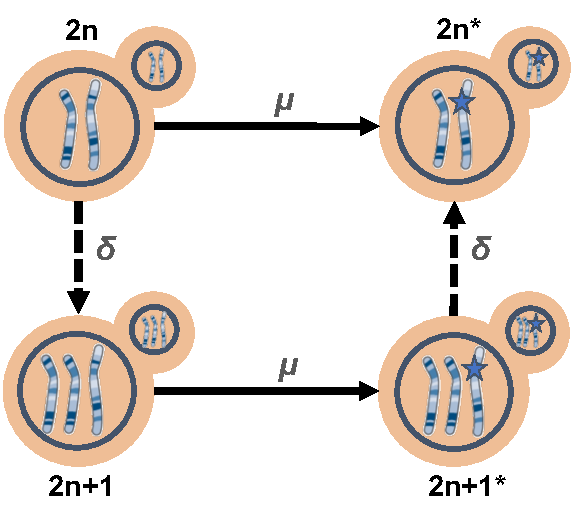
\includegraphics[height=1.8in]{../figures/Fig1-A.pdf}      
      \label{fig:model1}
  \end{subfigure}%
  \\
  \begin{subfigure}[t]{0.5\textwidth}
  	  \caption{
        \textbf{B. Multi-locus model}
      }
      \centering
      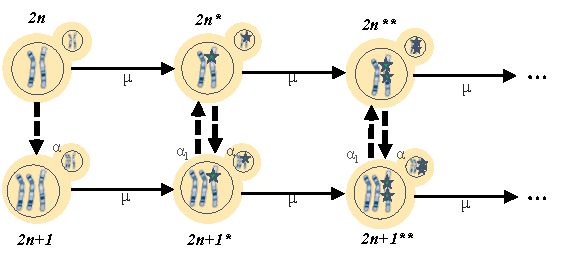
\includegraphics[height=1.8in]{../figures/Fig1-B.pdf}      
      \label{fig:model2}
  \end{subfigure}
  \caption{
    \textbf{Model illustrations.}
    \textbf{(A)} In the single-locus model, the four genotypes are: euploid wild-type, \euwt; euploid mutant, \eumt; aneuploid wild-type, \anwt; and aneuploid mutant, \anmt.
    Overall there are two possible trajectories from \euwt to \eumt.
    \textbf{(B)} In the multi-locus model, each genotype is characterized by its karyotype, \euwt or \anwt, and the number of accumulated beneficial mutations, denoted by stars. 
    In both panels arrows denote transitions between genotypes, with transitions rates: $\mu$, mutation rate; $\delta$, aneuploidy gain rate; $\delta_L$, aneuploidy loss rate.
  }
  \label{fig:models}
\end{figure}

\paragraph*{Evolutionary Models.}
We developed two models: a single-locus model and a multi-locus model. 
Both models are based on the Wright-Fisher model~\citep{Otto2007}, assuming non-overlapping generations and including the effects of natural selection, genetic drift, aneuploidy, and mutation. 
We focus on beneficial mutations, neglecting the effects of deleterious and neutral mutations. Both models allow for a single aneuploid karyotype (e.g., chromosome III duplication).
While the single-locus model allows for only a single mutation to occur, the
multi-locus model allows for multiple mutations to accumulate in the genome~(\autoref{fig:models}).

\paragraph*{Single-locus model.}
This model assumes a constant population size $N$ and follows four genotypes~(\autoref{fig:models}A): euploid wild-type, \euwt, the initial genotype; 
euploid mutant, \eumt, with the standard karyotype and a single beneficial mutation; 
aneuploid wild-type, \anwt, with an extra chromosome, e.g. following chromosome duplication; and
aneuploid mutant, \anmt, with and extra chromosome and a beneficial mutation. 

Transitions between the genotypes occur as follows~(\autoref{fig:models}A): Beneficial mutations from \euwt\; to \eumt\; occur with probability $\mu$, the mutation rate, and from \anwt\; to \anmt\; with probability $\tau \mu$, where $\tau$ is the fold-change in the rate of beneficial mutations in aneuploid cells. By default, we assume $\tau=33/32$, as the wild-type \yeast strains in the experiments by \citep{Yona2012} are diploid, with 32 chromosomes, and the aneuploid strains are trisomic, with 33 chromosomes.
Aneuploidy is formed by chromosome mis-segregation, so that cells transition from \euwt\; to \anwt\ with probability $\delta$, the aneuploidy gain rate.
Aneuploidy is lost, transitioning cells from \anmt\; to \eumt\; with probability $\delta_L$, the aneuploidy loss rate.
The fitness values of the four genotypes are given by \autoref{table:single-locus}.

%%% Table: single-locus model
\begin{table}[h]
\centering
\caption{\textbf{Single-locus model fitness values.}}
\begin{tabular}{lllll}
\emph{Genotype} $i$ & $2n$ & $2n+1$ & $2n+1^*$ & $2n^*$ \\
\hline
\emph{Fitness} $w_i$ & $1$ & $1-c+b$ & $(1-c)(1+s)+b$ & $1+s$               
\end{tabular}
\label{table:single-locus}
\caption*{
$s \ge 0$ is the selection coefficient of a beneficial mutation;
$b \ge 0$ is the selection coefficient of aneuploidy; 
and $0 \le c \le 1$ is the fitness cost of aneuploidy.
}
\end{table}
%%%

The first generation is initialized with $N$ cells with genotype \euwt.
The effect of natural selection on the frequency $f_i$ of genotype $i = 2n, 2n+1, 2n+1^*, \text{or } 2n^*$ is given by
    \begin{equation} \label{eq:selection-single} 
      f^s_i = \frac{f_i w_i}{\bar{w}} \;,
    \end{equation}
where the fitness values $w_i$ are given in \autoref{table:single-locus} and $\bar{w} = \sum_{j}{f_j w_j}$ is the population mean fitness.
The effect of mutation and aneuploidy on genotype frequencies is given by
    \begin{equation} \label{eq:mutation-aneuploidy-single}
    \begin{aligned}
      &f^m_{2n} &=&\; (1 - \delta - \mu) f^s_{2n}  \;,\\
      &f^m_{2n+1} &=&\; \delta f^s_{2n} + (1 - \tau \mu) f^s_{2n+1}  \;,\\
      &f^m_{2n+1^*} &=&\; \tau \mu f^s_{2n+1} + (1-\delta_L) f^s_{2n+1^*}  \;,\\
      &f^m_{2n^*} &=&\; \mu f^s_{2n} + \delta_L f^s_{2n+1} + f^s_{2n^*}  \;.
    \end{aligned}
    \end{equation}
Finally, random genetic drift is modeled using a multinomial distribution~\citep{Otto2007},
    \begin{equation} \label{eq:drift-single}
      \vec{f'} \sim \frac{1}{N} Mult(N, \vec{f^m}) \;,
    \end{equation}
where $\vec{f^m}=(f^m_{2n},f^m_{2n+1},f^m_{2n+1^*},f^m_{2n^*})$ are the frequencies of the genotypes after mutation and aneuploidy, $\vec{f'}$ are the genotype frequencies in the next generation, and $Mult(N, \vec{f})$ is a multinomial distribution parameterized by the population size $N$ and the genotype frequencies $\vec{f}$.
Overall, the change in genotype frequencies from one generation to the next is given by the transformation $f_i \to f'_i$.

\paragraph*{Multi-locus model.}
This model expands the single-locus model by allowing for (i) the accumulation of beneficial mutations in the genome, and (ii) a fluctuating population size. 

A genotype is characterized by its karyotype, \euwt\; or \anwt, and the number of accumulated beneficial mutations, which can be zero or more.
The selection coefficient of the $i$-th accumulated mutation in each individual, $s_i$, is drawn from an exponential distribution with expected value $s$, $s_i \sim Exp(s)$.
The rest of the parameters ($N$, $\mu$, $\tau$, $\delta$, $\delta_L$, $b$, $c$) are the same as in the single-locus model.
% ILIA: I don’t know if it should be mentioned here, but the meaning of the mutation rate is a bit differ for multi-locus model. For the single-locus mutation rate value is the probability to get specific mutation (maybe one of a few). For the multi-locus it is the probability to get some beneficial mutation (one of a many). So, we don’t expect to receive same values for mutation rate for the models.
% ILIA: I don’t have in the code 𝜏 parameter for multi-locus model (it’s like 1 there). Do you think it worth adding it for consistency?
The fitness of the different genotypes is the same as in the single-locus model (\autoref{table:single-locus}), except that the fitness contribution of $k$ beneficial mutations is the product of their independent effects, $\prod_{i=1}^k(1+s_i)$, instead of the contribution of the single mutation allowed in the single-locus model, $(1+s)$, see \autoref{table:multi-locus}.
Therefore, aneuploidy loss would be favored by selection only if there are enough beneficial mutations and/or the selection coefficients $s_i$ are large enough. The intuition is that when the benefit of the accumulated beneficial mutations is small, the benefit of aneuploidy has a large effect; when the benefit of the accumulated beneficial mutations benefit is large, then aneuploidy is no longer advantageous because of its significant cost.

In contrast to the single-locus model, in the multi-locus model the population size changes in order to model serial-transfer experiment protocol~\citep{Yona2012}: the population is serially diluted by transferring a fraction of the population (1/120) to a fresh medium, starting a new growth cycle.
In this model, the population initial size is $N_0 = N$, and the population size is doubled every generation, $N_1=2N, N_2=4N, \ldots$, and diluted back to $N$ every eight generations, $N_8=N$.

The change in frequencies due to selection is exactly the same as in the single-locus model (\autoref{eq:selection-single}), only applied using the fitness values in \autoref{table:multi-locus}. The change due to random genetic drift is also the same as in \autoref{eq:drift-single}, except that the frequencies vector is $\vec{f}=(f_{2n}, f_{2n+1}, f_{2n^*}, f_{2n+1^*}, f_{2n^{**}}, f_{2n+1^{**}}, \ldots)$ and that the population size changes between generations, as described above.

The effects of mutation and aneuploidy on genotype frequencies is more elaborate than in the single-locus model.
Genotype $i$ is classified according to their karyotype (\emph{2n} or \emph{2n+1}), the number of accumulated beneficial mutations ($k \ge 0$), and their fitness ($w_i$).
Each offspring cell inherits these properties from its mother cell.
Then, with probability $\mu$ or $\tau \mu$ for euploid and aneuploid cells, respectively, a new beneficial mutation is accumulated, such that the number of mutations is $k+1$, and its effect $s_{k+1}$ is drawn from an exponential distribution with expected value $s$, such that the contribution of the mutations to the fitness is $\prod_{j=0}^{k+1}{(1+s_j)}$.
Next, euploid offspring become aneuploid with probability $\delta$, and aneuploid offspring become euploid with probability $\delta_L$.

%%% Table: multi-locus model
\begin{table}[h]
\centering
\caption{\textbf{Multi-locus model fitness values.}}
\begin{tabular}{lllll}
\emph{Genotype} $i$ & $2n$ & $2n+1$ & $2n+1^{*k}$ & $2n^{*k}$ \\
\hline
\emph{Fitness} $w_i$ & $1$ & $1-c+b$ & $(1-c)\prod_{j=1}^k(1+s_i)+b$ & $\prod_{j=1}^k(1+s_i)$               
\end{tabular}
\label{table:multi-locus}
\caption*{
$k$ is the number of accumulated beneficial mutations in the genome;
$s \ge 0$ is the selection coefficient of a beneficial mutation;
$b \ge 0$ is the selection coefficient of aneuploidy; 
and $0 \le c \le 1$ is the fitness cost of aneuploidy.
}
\end{table}
%%%

\paragraph{Empirical evidence.}
Our inference procedure uses empirical data from evolutionary experiments performed by \citet{Yona2012}.
In the heat-stress experiment, four populations of \yeast evolved under \SI{39}{\celsius}. Aneuploidy fixed in all four population in the first 450 generations (hereafter, fixation or elimination of a genotype by generation $t$ means that more than 95\% or less than 5\% of the population carry the genotype at generation $t$, and possibly earlier).
The experiment continued with two populations, in which aneuploidy was eliminated by generation 1700 and 2350.
In the pH-stress experiment, four populations of \yeast evolved under high-ph stress (8.6). Aneuploidy fixed during the first 150 generations. It was fully eliminated in two populations and partly eliminated in two populations by generation 750. 
These empirical results were published by \citet{Yona2012}.

\paragraph{Likelihood function.}
Denote by $A_{t}$ the fixation of aneuploidy at generation $t$, by $L_{t}$ the loss of aneuploidy at generation $t$, and by $L^*_{t,T}$ the loss of aneuploidy at generation $t$ conditioned on no loss by generation $T$.
The model likelihood function for parameter vector $\theta$ for the heat-stress experiment is
\begin{multline} \label{eq:heatstress-likelihood}
\likelihood(\theta | A_{450}, L_{1700}, L^*_{2350, 1700} ) = \\
P^4(A_{450}) \cdot \Big(1 - P^4(\lnot{L_{1700}} | A_{450} ) - P^4(\lnot{L^*_{2350, 1700}}| A_{450}) + P^4(\lnot{L_{1700}} \land \lnot{L^*_{2350, 1700}}| A_{450})\Big)	\;,	
\end{multline}
where $P(X)$ is the probability of event $X$ and $\lnot$ means \emph{not}. 

The likelihood function of the model with parameter set $\theta$ for the pH-stress experiment is
\begin{equation} \label{eq:phstress-likelihood}
\likelihood(\theta | A_{150}, L_{750} ) = \\
 P^4(L_{450}) \cdot 6 \cdot	P^4(L_{750} | A_{150}) \cdot P^4(\lnot{L_{750}} | A_{150}) \;.  
 \end{equation} 
%TODO i think it is wrong because fig 5C shows that only 2 replicas are fixated after 650 generations (see Supplementary also) Anyway, I don't think that we use this likelihood, so probably should be removed at all.
 
For the model without aneuploidy let's denote by $M_{t}$ the fixation of \eumt at generation $t$, and by $M^*_{t,T}$ the fixation of \eumt at generation $t$ conditioned on no fixation at generation $T$.
The likelihood of the model without aneuploidy with parameter vector $\theta$ for the heat-stress experiment is
\begin{multline} \label{eq:heatstress-noaneuploidy-likelihood}
\likelihood(\theta |  M_{1700}, M^*_{2350, 1700} ) = \\
\Big(1 - P^4(\lnot{M_{1700}}) - P^4(\lnot{M^*_{2350, 1700}}) + P^4(\lnot{M_{1700}} \land \lnot{M^*_{2350, 1700}})\Big)	\;,	
\end{multline}

Because of the complexity of the model, this likelihood function is intractable. Therefore, given specific values of the model parameters $\theta$, we simulate the model in many replicates to approximate the value of the likelihood function $\likelihood(\theta)$.

\paragraph{Parameter inference.} To infer model parameters, we use approximate Bayesian computation~\citep{Sunnaker2013} with a sequential Monte-Carlo scheme, or ABC-SMC~\citep{Sisson2009}, implemented in the \texttt{pyABC}\footnote{https://pyabc.readthedocs.io} Python 
package~\citep{Klinger2018}.
Briefly, this approach uses numerical stochastic simulations of the model to infer a posterior distribution over the model parameters. It is a method of likelihood-free, simulation-based inference~\citep{Cranmer2020}, that is, for estimating a posterior distribution when a likelihood function cannot be computed. It is therefore suitable to our case, in which the likelihood function can only be approximated from simulations, and cannot be directly computed. 
After getting weighted particles of the posterior distribution using ABC-SMC scheme, we calculate Kernel Density Estimate using Gaussian kernels. $50,000$ sampled points from KDE represent the posterior distribution over the model parameters, and we use it for plots, median calculation, etc.
% TODO ILIA please add all configuration details, similar to the relevant section in the NPI paper. Discuss priors, convergence tests, etc.
% And also number of replicates for different models

\paragraph{Prior distributions.} The prior distributions of $w_{2n+1}=1-c+b$, $w_{2n+1^*}=(1+s)(1-c)+b$ and $w_{2n^*}=1+s$ were obtained by estimating it from growth curves data that were previously obtained by~\citet{Yona2012} using mono-culture growth experiments.
The raw growth curves data were not published before, but were used to produce figures 3C, 4A, and S2 in \citet{Yona2012}.
We used \texttt{Curveball}\footnote{https://curveball.yoavram.com}, a dedicated method for predicting results of competition experiments from growth curve data~\citep{Ram2019}. \texttt{Curveball} takes growth curves of two strains growing separately in mono-culture and predicts how they would grow in a mixed culture, that is, it predicts the results of a competition assay.
From these predictions, relative fitness values can be computed.  

We used growth curves of $2n+1$ and $2n$ in \SI{39}{\celsius} to estimate  $w_{2n+1}$. We used the same prior for $w_{2n+1^*}$ and $w_{2n^*}$, assuming that fitness values shouldn't be differ too much. We also tested different priors, but this one (let's call it main prior) was better in sense of WAIC, prediction plots, estimated parameters. %TODO provide formula of WAIC. Table? To show ppc plots also?. 
\\We tested uninformative uniform prior, $\mathit{Uniform}(1,6)$, for all $w_{2n+1}$, $w_{2n+1^*}$, $w_{2n^*}$ and only for $w_{2n+1^*}$, $w_{2n^*}$, leaving $w_{2n+1}$ prior as before . In both scenarios the estimated by the model parameters of fitness were looks too high: for the first scenario the estimated medians were  $w_{2n+1}=2.767$, $w_{2n+1^*}=5.79$, $w_{2n^*}=5.827$ and for the second $w_{2n+1}=1.046$, $w_{2n+1^*}=4.642$, $w_{2n^*}=4.684$. We don't expect to have such high fitness values. Moreover the WAIC for the models with these priors are 0.57 and 1.9 respectively, while WAIC for the main prior model is 0.27. Also for the model with uninformative prior for all $w_{2n+1}$, $w_{2n+1^*}$, $w_{2n^*}$ the fixation time of 2n+1 is about 16 in average, that contradicts unpublished observations that were about 250-300.
\\Also we tried to use additional growth curves. We used growth curves of 2n* (\emph{refined} from \citet{Yona2012}) and 2n+1 in \SI{39}{\celsius} to estimate $w_{2n*}/w_{2n+1}$. The same prior was used for $w_{2n*}/w_{2n+1*}$. This model didn't perform well, resulted in WAIC 2.8.
\\Another try was to use growth curves of $2n+1$ and $2n$ in \SI{30}{\celsius} to estimate $1-c$. This estimation assumes that the cost of aneuploidy is the same in \SI{39}{\celsius} and \SI{30}{\celsius}; this might be incorrect, but we only assumed this to generate a prior distribution for the fitness values. The prior for $b$ was taken the same as for $c$. This model didn't work at all: we didn't receive any parameter that the likelihood with it is greater than zero. %TODO it make sense because bla bla?
 
Because \texttt{Curveball} uses a maximum-likelihood approach to estimate model parameters, we were able to estimate a distribution of relative fitness values by sampling from a truncated multivariate normal distribution defined by the maximum-likelihood covariance matrix. Thus, we sampled 10,000 values for appropriate fitness, which we used as prior distributions. 
See Figures~\ref{fig:growth-curves-30deg} and~\ref{fig:growth-curves-39deg}.

For the mutation rate $\mu$ and aneuploidy rate $\delta$ we used uniform priors, $\mathit{Uniform}(1e-8,1e-5)$ and $\mathit{Uniform}(1e-6,1e-3)$ respectively. We have tried also uniform priors with lower than $1e-8$ bound for $\mu$, but anyway the posterior ends with higher values. 
For the single locus model without aneuploidy, for the mutation rate wider uniform prior was used - $\mathit{Uniform}(1e-10,1e-5)$. 
%TODO ILIA please report here the point estimate and 95% CI for the three distributions, I only have for 1-c+b: 0.9863 (95% CI 0.9790 - 0.9939).
%TODO ILIA describe the priors for the mutation and aneuploidy rate.
% TODO also describe the prior for the model without aneuploidy - the mutation rate is wider here.

\paragraph{Model comparison.}  % TODO ILIA what did you do for model comparison/selection? 

\pagebreak
% Results
\section*{Results}

\subsection*{Model fitting}

%\paragraph{Simple model: Inference.}
%tell point estimates (+- hdi) (fig 2 from poster, add hdi)
%posterior predictions, sensitivity analysis
%time to fixation of aneuploidy 2n+1 - fits unpublished data
%figures
%- posterior distributions
%- expected frequency over time (fig 1 from poster)
%- % simulations to reach 2n+1, 2n*. (fig 3 from poster)
%- time to 2n* cannot be explained without aneuploidy (fig 4 from poster)
%- sensitivity analysis (fig 5 from poster)
%- convergence/ess of pyabc? 
%  - plot of posterior in each iteration shows convergence; 
%  - robustness of posterior to initial conditions - MAP+-HDI for different seeds;

\paragraph{Single-locus model parameters inference.} 
First we inference the parameters of the single-locus model. The mean and credible interval (2.5th percentile and the 97.5th percentile) of the parameters are:
mutation rate - $1.02\substack{+2.40 \\ -1.34}\times10^{-6}$,
trisomy rate - $7.36\substack{+3.55 \\ -4.82}\times10^{-4}$,
2n+1 fitness - $1.022\substack{+0.004 \\ -0.004}$,
2n+1* fitness - $1.025\substack{+0.004 \\ -0.004}$,
2n* fitness - $1.028\substack{+0.004 \\ -0.004}$.
This trisomy rate appropriates to the previous estimates; The mutation rate corresponds to the mutations target size of $10^{4}$ if we assume the mutation rate of single base to be about $2*10^{-10}$ as in previous estimates ~\citep{Zhu2014}. 
We can see from the posterior distribution~(\autoref{fig:posterior}) the correlation between fitness of different genotypes (\anwt, \anmt, \eumt)..(TODO say/plot something about the correlation, is it interesting?). 

\begin{figure}[h!]
  \centering
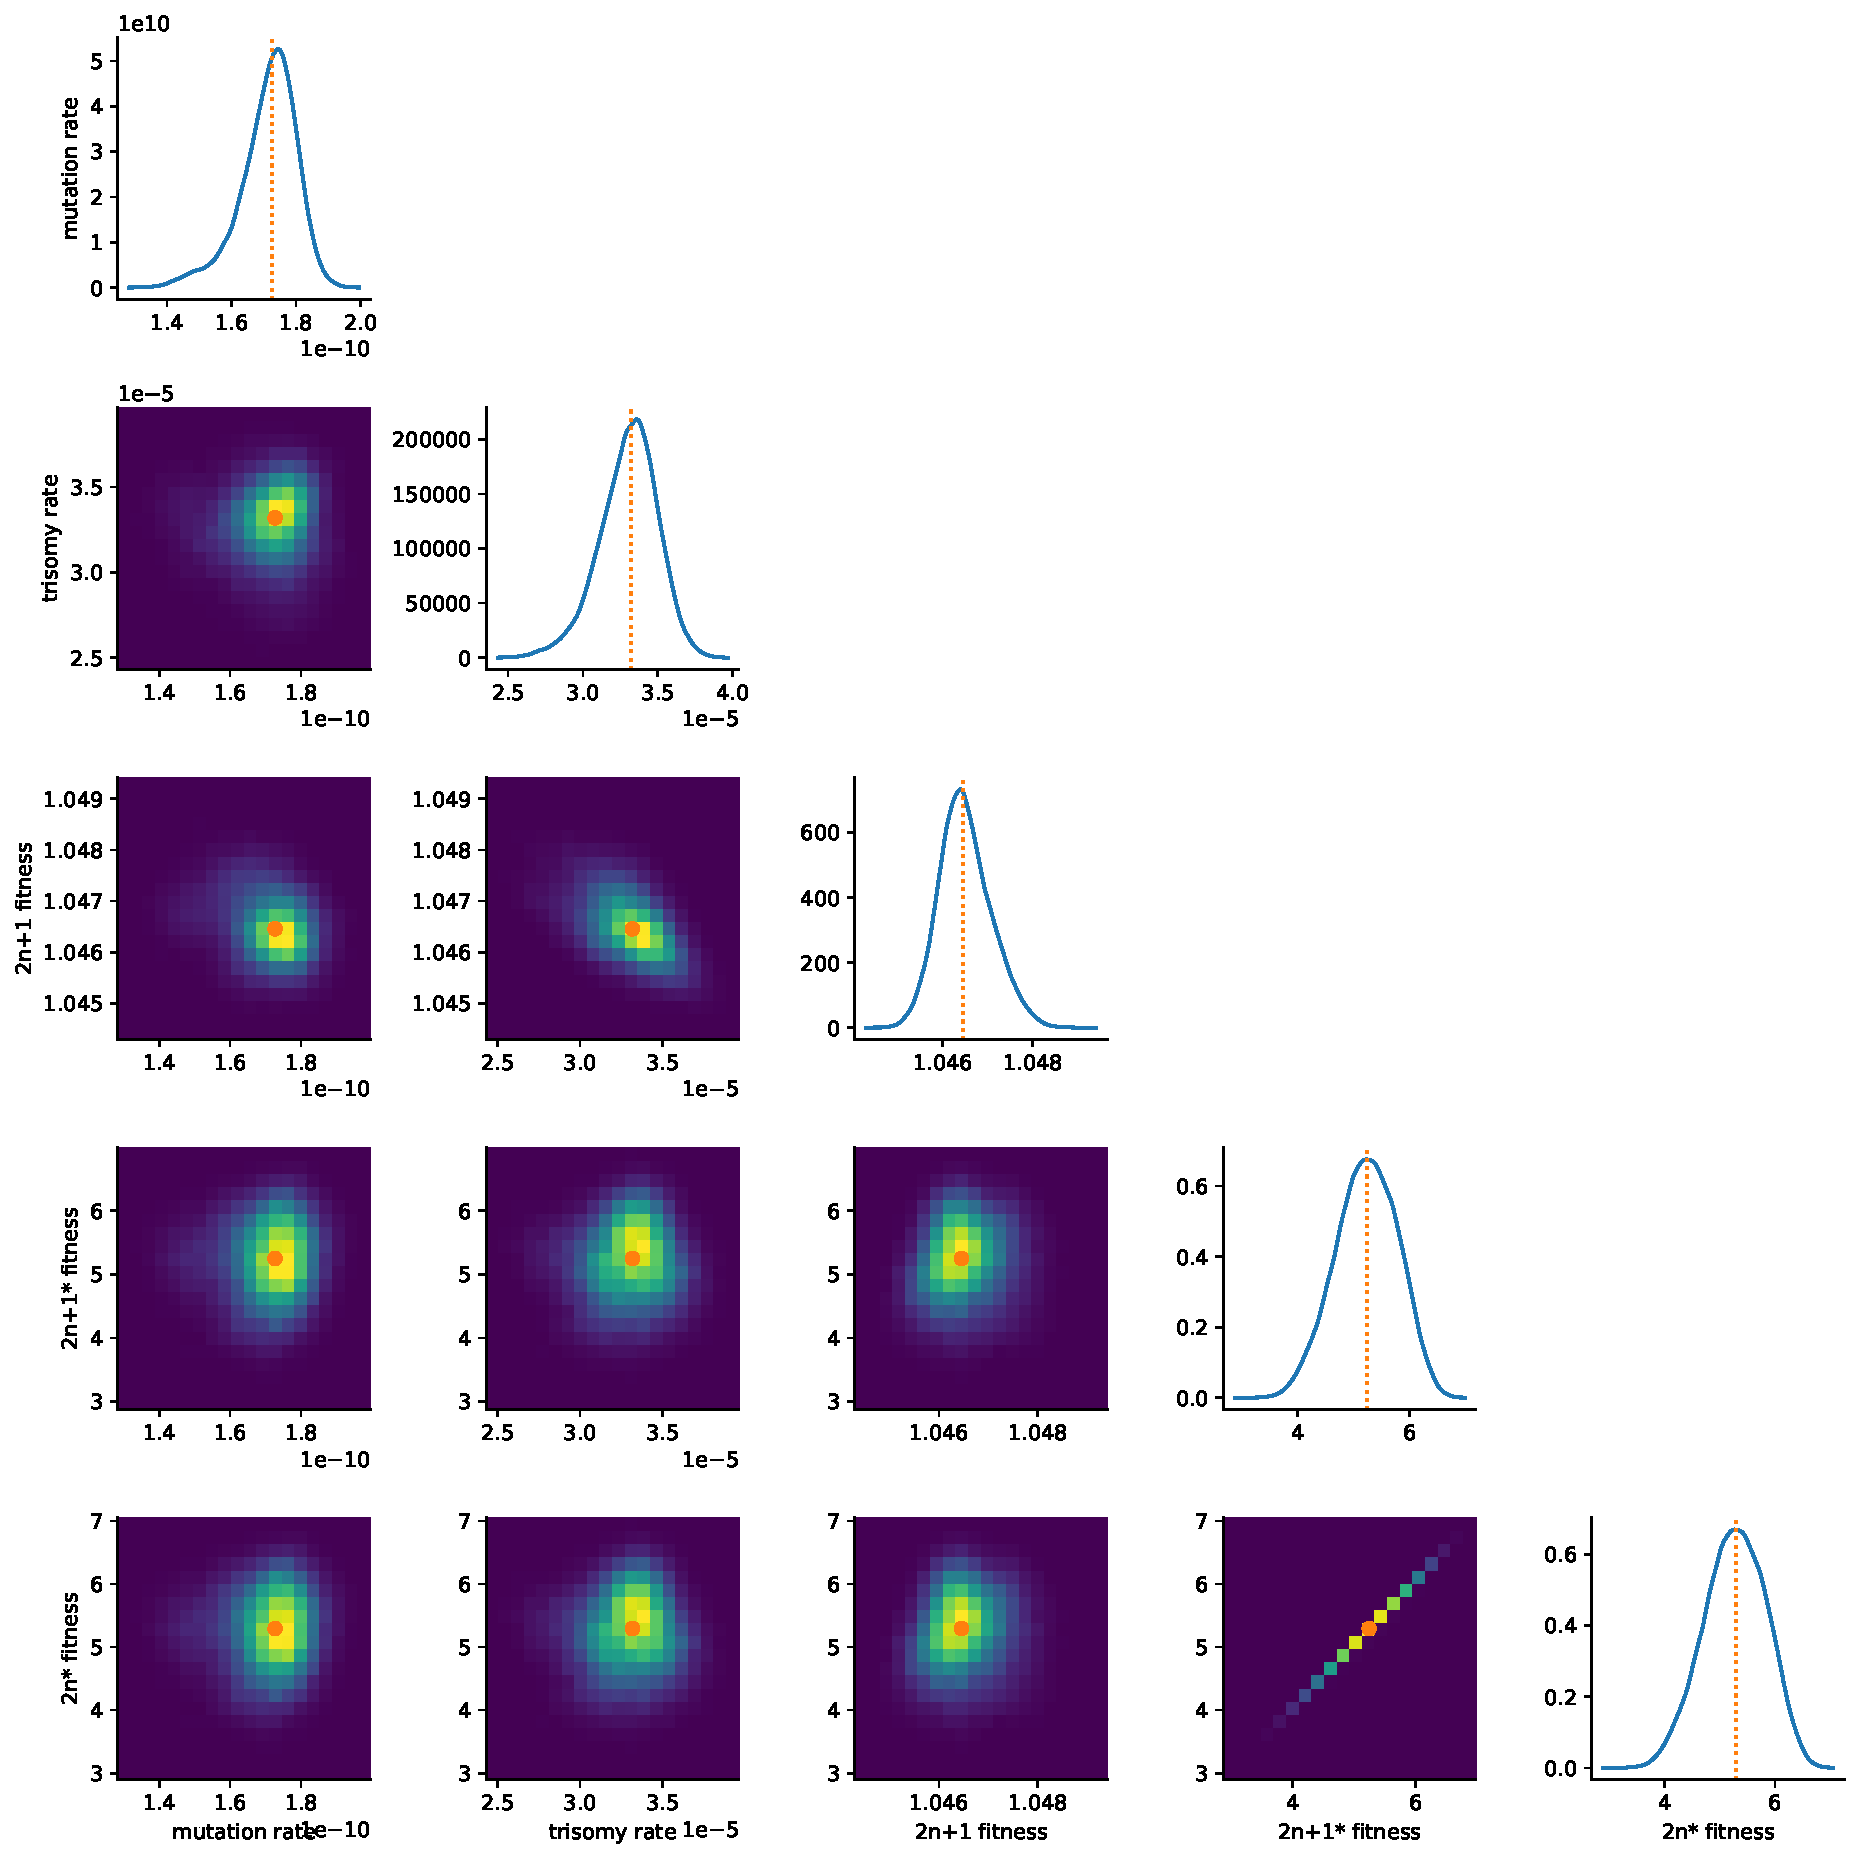
\includegraphics[width=0.9\textwidth]{../figures/posterior.pdf}
  \caption{
  \textbf{Single-locus model parameters posterior density.}
%TODO histogram on diagonal
The posterior density for each parameter is presented on the diagonal plots. Other plots represent joint posterior density of two parameters where blue color has the lowest density and yellow has the highest density. Red point and the dashed lines represent the median (TODO check that it is median and not mean) values of the densities: 
mutation rate - $1.02\times10^{-6}$,
trisomy rate - $7.36\times10^{-4}$,
\anwt fitness - $1.022$,
\anmt fitness - $1.025$,
\eumt fitness - $1.028$.
  } 
  \label{fig:posterior}
\end{figure}

\paragraph{Single-locus model fits the data well, but only if contains aneuploidy.} Single-locus model provide good fit to the data~(\autoref{fig:likelihood}A).
On \autoref{fig:ppc-plot} the dynamics of frequency change of each genotype in time is shown. We can see that \anmt never reach substantial frequency in the population.  
Sensitivity analysis~(\autoref{fig:sensitivity}) shows that if we change the parameter values the fit degrades. Furthermore, we measured fixation time of \anwt in population, and found it appropriate to the unpublished data of the experiment ~\citep{Yona2012} - about 300 generations in average.
On the other hand, if we don't take into consideration aneuploidy in the model, i.e. take aneuploidy rate be equal to zero, then the model can't explain the data: the fit is not so good~(\autoref{fig:likelihood}A; \autoref{fig:2n*-fixation}). The good fit of the model without aneuploidy to the data, requires much lower mutation rate (TODO provide numbers for the median fit?). If mutation rate is not low, the fixation of \eumt happens much quicker (see yellow and blue bars at  \autoref{fig:2n*-fixation}).

\begin{figure}[h!]
  \centering
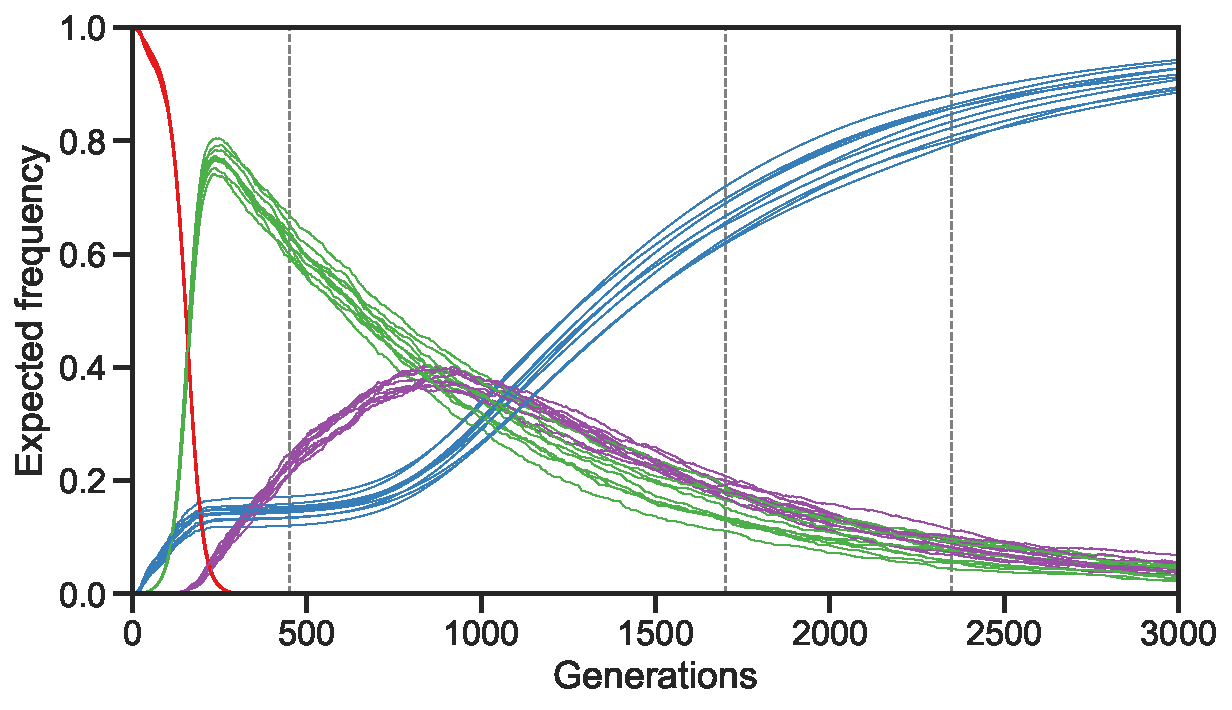
\includegraphics[width=0.6\textwidth]{../figures/ppc-plot.pdf}
  \caption{
  \textbf{Evolutionary dynamics with fitted single-locus model.} 
  Frequency of the four genotypes averaged over 10,000 simulations of the model. Each line represent one of the 10 parameter sets drawed from the inference posterior.
  }
  \label{fig:ppc-plot}
\end{figure}

\begin{figure}[h!]
  \centering
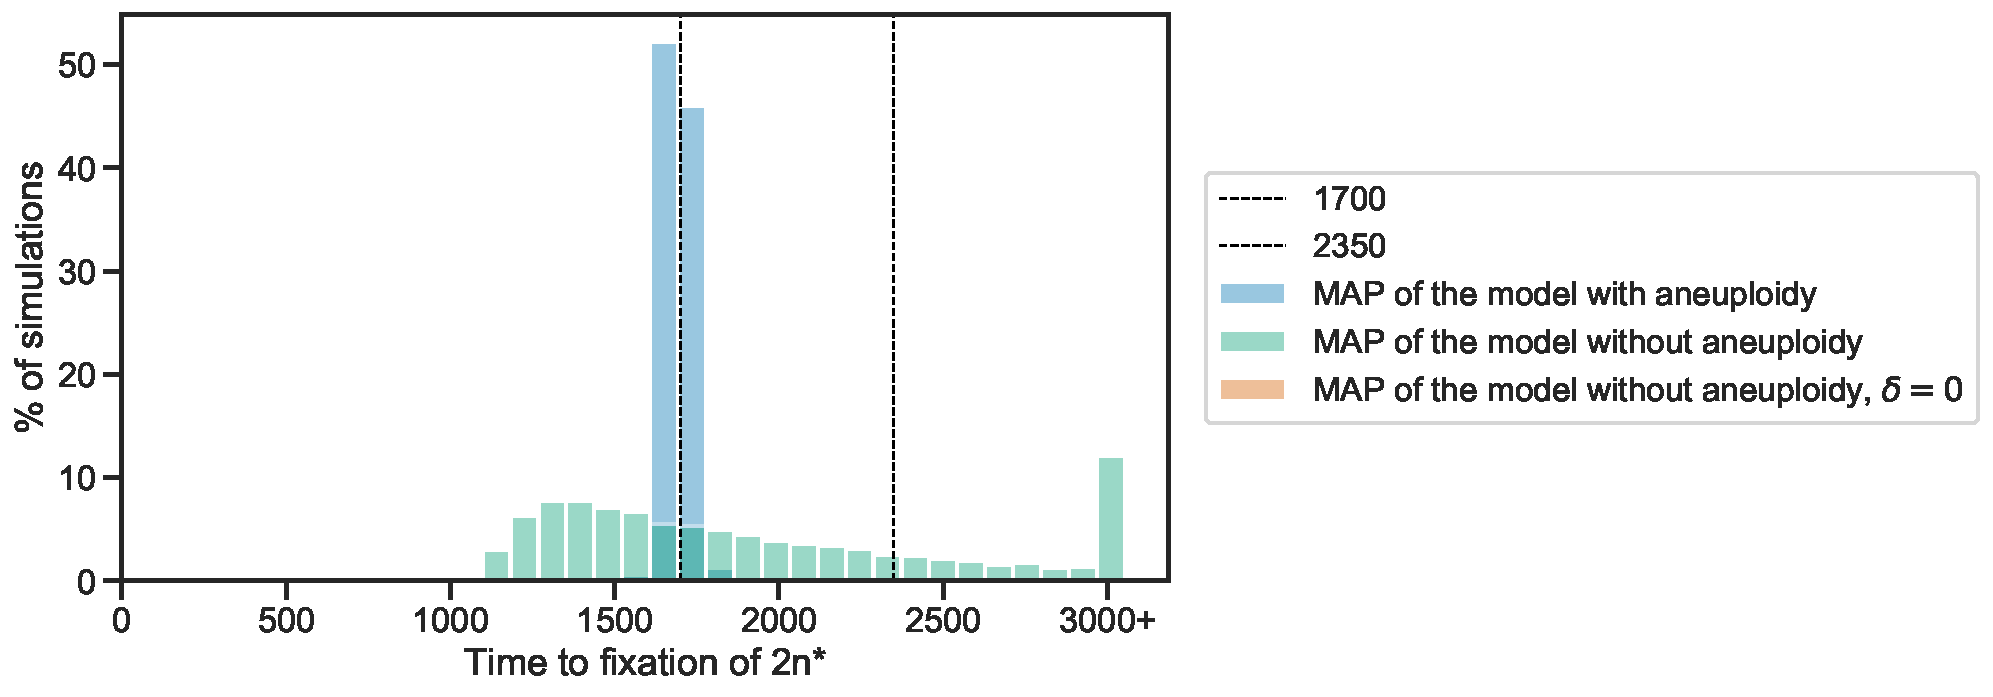
\includegraphics[width=0.6\textwidth]{../figures/fixation-plot.pdf}
  \caption{
  \textbf{Time of \eumt fixation cannot be explained without aneuploidy.}
Each color represents distribution to fixation of \eumt of $10,000$ simulations for different modifications of single-locus model. \emph{Blue} represents the model with aneuploidy with parameters that taken from posterior median when we fit the model to the experimental data. \emph{Orange} represents the same model that have no aneuploidy, i.e aneuploidy rate is zero. \emph{Green} represents the model without aneuploidy with parameters that taken from posterior median when we fit the model without aneuploidy to the experimental data. The last bin contains all the simulations with time greater than 3000.
Dashed lines show experimental data: generations 1700 and 2350. The fit to the data is better when the distribution is such that the difference in number of simulations in ranges 0-1700 and 1700-2350 is small and there's no many simulations after 2350 generations. The fit of \emph{blue} is better than of \emph{green}. And there's no fit of \emph{red} to the data at all.
  }
  \label{fig:2n*-fixation}
\end{figure}

\paragraph{Complex model: Inference and Comparison.}

%same for complex model
%model comparison between models - model probabilities

\pagebreak
% Discussion
\section*{Discussion}

\paragraph*{Aneuploidy is not just another type of mutation.}
The published data indicate that, like mutation, aneuploidy can be both deleterious and beneficial~\citep{Pavelka2010, Sheltzer2011}.
Nevertheless, there are important and fundamental differences between adaptation by aneuploidy
and adaptation by beneficial mutations~\citep{Yona2015}, which make aneuploidy a unique mechanism for generating genetic
variation.
First, the aneuploidy rate (i.e. the frequency of mis-segregation events) is significantly higher than the
mutation rate~\citep{Santaguida2015review}.
Thus, everything else being equal, adaptation by aneuploidy will be faster and more frequent.
Second, fitness effects of aneuploidy are larger than those of the majority of mutations, on average, and are rarely
neutral~\citep{Pavelka2010, Yona2012, Sunshine2015}, allowing selection to quickly sort deleterious and beneficial genotypes.
Third, the number of different karyotypes is considerably smaller than the number of different genotypes, and different karyotypes are likely to have different phenotypes~\citep{Pavelka2010}.
Therefore, exploration of the phenotype space by aneuploidy requires smaller populations and a shorter time span.
Fourth, aneuploidy is a reversible state, as the rate of chromosome loss is high and the cost of aneuploidy is significant~\citep{Niwa2006}.
Indeed, aneuploidy often provides a transient solution: under short-term stress conditions, aneuploidy reverts (chromosome number returns to normal) when the stress subsides; under long-term stress conditions, aneuploidy reverts when refined solutions, generated by beneficial mutations, take over~\citep{Yona2012}.
Finally, aneuploidy results in increased genome instability, potentially increasing genetic variation by a positive feedback loop~\citep{Rancati2013, Bouchonville2009, Zhu2012}, while also increasing its own transience.

\paragraph*{Evolutionary theory of aneuploidy.}
The role of aneuploidy in adaptation has only recently been observed~\citep{Sionov2010, Yona2012, Gerstein2015}, and is largely missing from the literature on evolution and adaptation:
the introductory textbook \emph{Evolution} by~\citet{Bergstrom2012} does not mention the word aneuploidy, and the graduate-level book \emph{Mutation-Driven Evolution} by~\citet{Nei2013} only briefly mentions aneuploidy in the context of speciation, but not adaptation.
In recent reviews of the literature, aneuploidy is suggested to play an important role in fungal adaptation~\citep{Robbins2017, Todd2017} and cancer evolution~\citep{Santaguida2015review, Naylor2016, Sansregret2017}, yet these reviews cite no theoretical studies nor any quantitative models.
Indeed, evolutionary, ecological, and epidemiological studies mostly assume adaptation occurs via beneficial mutations, recombination, and sex.
Therefore, there is a critical need to develop an evolutionary theory of aneuploidy like the evolutionary theories of other mechanisms for generation of genetic variation, e.g. mutation~\citep{Lynch2010}, recombination~\citep{Hartfield2012}, and sex~\citep{Otto2009}.
An evolutionary theory of aneuploidy will be central to the interpretation of experimental and clinical observations and design of new hypotheses, experiments, and treatments~\citep{Carja2014}.
For example, despite the lack of theoretical models, aneuploidy has been invoked in a new strategy to combat pathogens and tumour cells by setting “evolutionary traps”~\citep{Gerstein2015,Chen2015}, in which a condition that predictably leads to emergence of aneuploidy is applied, followed by a condition that specifically selects against aneuploid cells.

\pagebreak
% Acknowledgements
{\small
\section*{Acknowledgements}
We thank Yitzhak Pilpel, Orna Dahan, Lilach Hadany, Judith Berman, David Gresham, Shay Covo, Martin Kupiec, and Tal Simon for discussions and comments.
This work was supported in part by 
the Israel Science Foundation (YR 552/19) and
Minerva Stiftung Center for Lab Evolution (YR).
}

\bibliographystyle{agsm}
\bibliography{ms.bib}

\section*{Supplementary Material}
\beginsupplement % https://support.authorea.com/en-us/article/how-to-create-an-appendix-section-or-supplementary-information-1g25i5a/



%%%% Fig - Curveball 30deg %%%
% generated with growth_curves.ipynb
\begin{figure}[h]
    \centering
	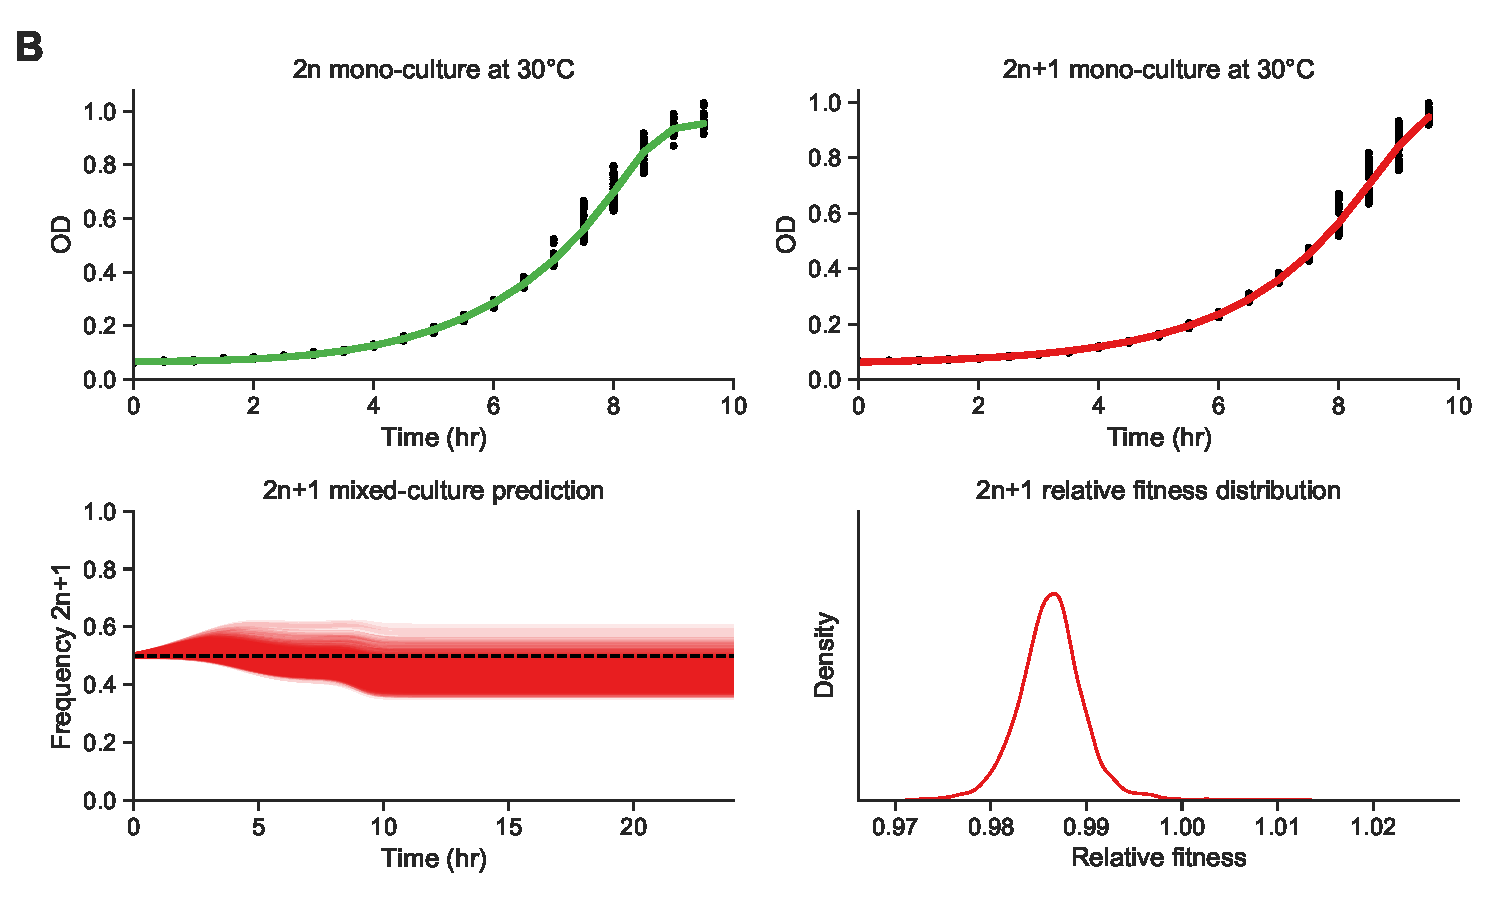
\includegraphics[width=0.5\textwidth]{../figures/evo39_fitness_30deg.pdf}
    \caption{
    \textbf{Fitness estimation from \SI{30}{\celsius}.}
    } 
    \label{fig:growth-curves-30deg}
\end{figure}

%%%% Fig - Curveball 39deg %%%
% generated with growth_curves.ipynb
\begin{figure}[h]
    \centering
	\includegraphics[width=0.5\textwidth]{../figures/evo39_fitness_39deg.pdf}
    \caption{
    \textbf{Fitness estimation from \SI{39}{\celsius}.}
    } 
    \label{fig:growth-curves-39deg}
\end{figure}

% likelihood plots
\begin{figure}[b!]
  \centering
  \begin{subfigure}[t]{0.5\textwidth}
      \caption{
        \textbf{A. With aneuploidy}
      }
      \centering
      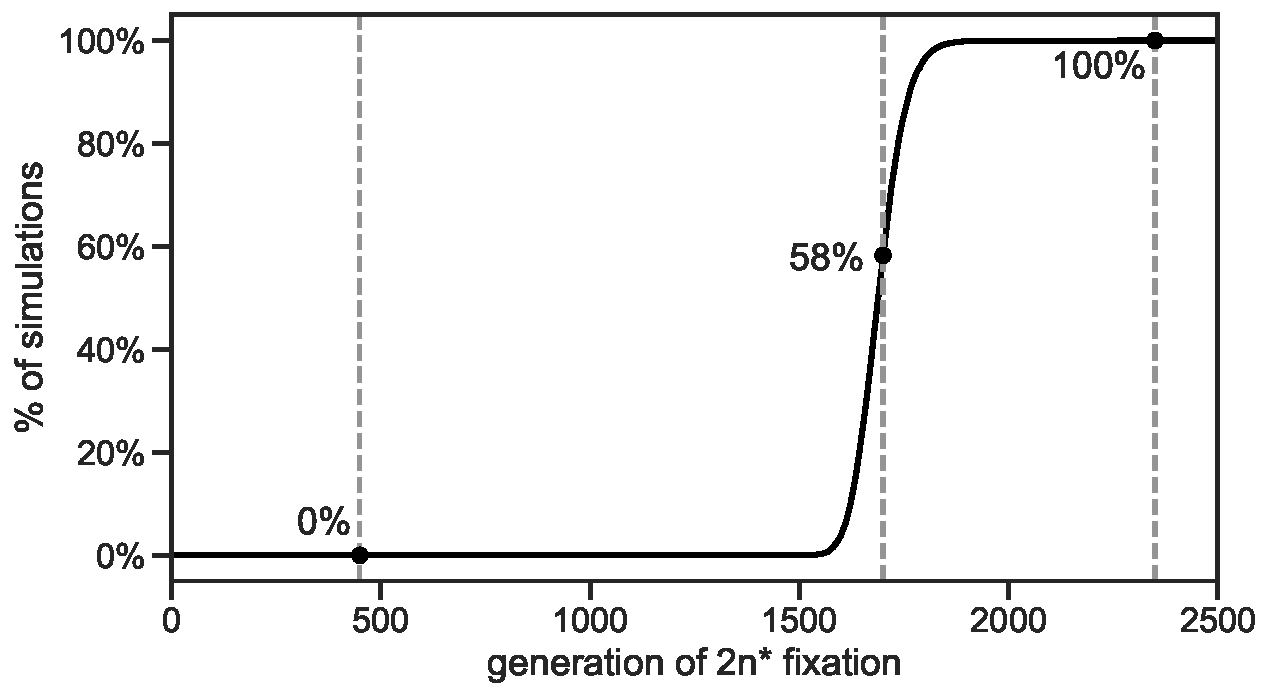
\includegraphics[height=1.8in]{../figures/likelihood-plot.pdf}      
      \label{fig:likelihood-with-aneuploidy}
  \end{subfigure}%
  \\
  \begin{subfigure}[t]{0.5\textwidth}
  	  \caption{
        \textbf{B. Without aneuploidy}
      }
      \centering
      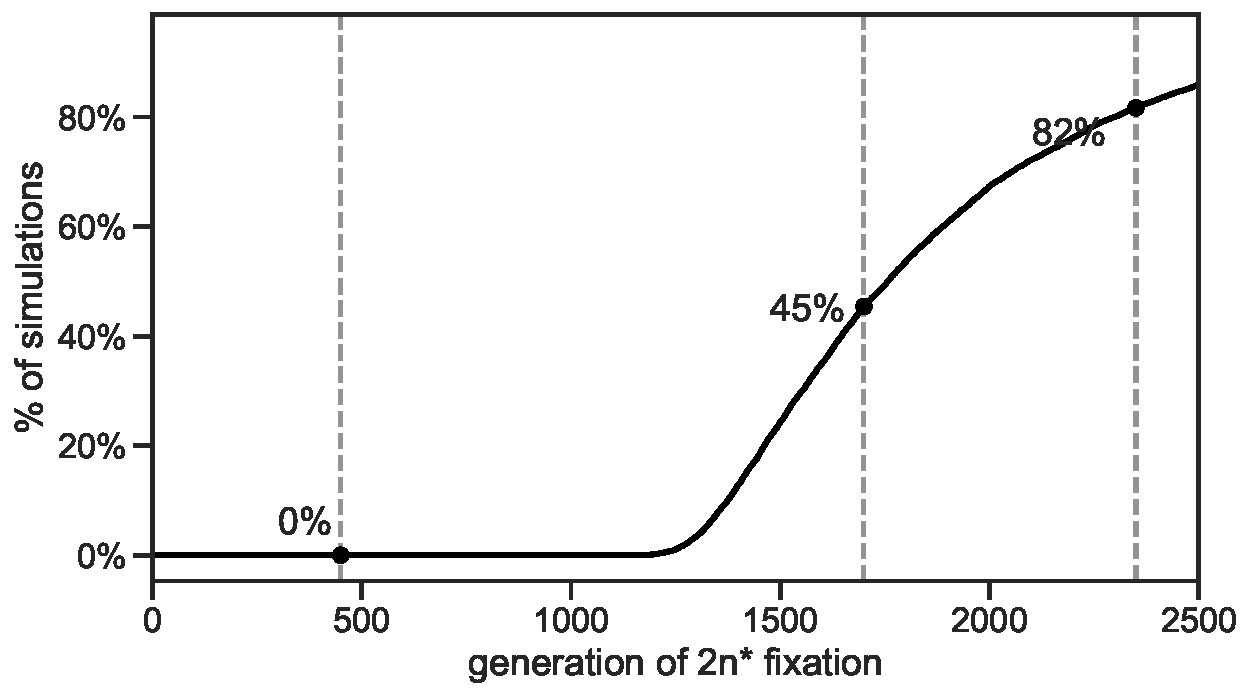
\includegraphics[height=1.8in]{../figures/likelihood-noaneuploidy-plot.pdf}      
      \label{fig:likelihood-without-aneuploidy}
  \end{subfigure}
  \caption{
    \textbf{Single-locus model fit.} Cumulative distribution of 10000 simulations are shown.
    \textbf{(A)} Simulations parameters are from the median of the posterior of the single-locus model fit. The likelihood for the heat-stress experiment (\autoref{eq:heatstress-likelihood}) is 0.86.
    \textbf{(B)} Simulations parameters are from the median of the posterior of the single-locus model \emph{without} aneuploidy fit. The likelihood for the heat-stress experiment (\autoref{eq:heatstress-noaneuploidy-likelihood}) is 0.75.
  }
  \label{fig:likelihood}
\end{figure}

% sensitivity analysis plots

\begin{figure}[p]
  \centering
  \begin{subfigure}{0.3\textwidth}
      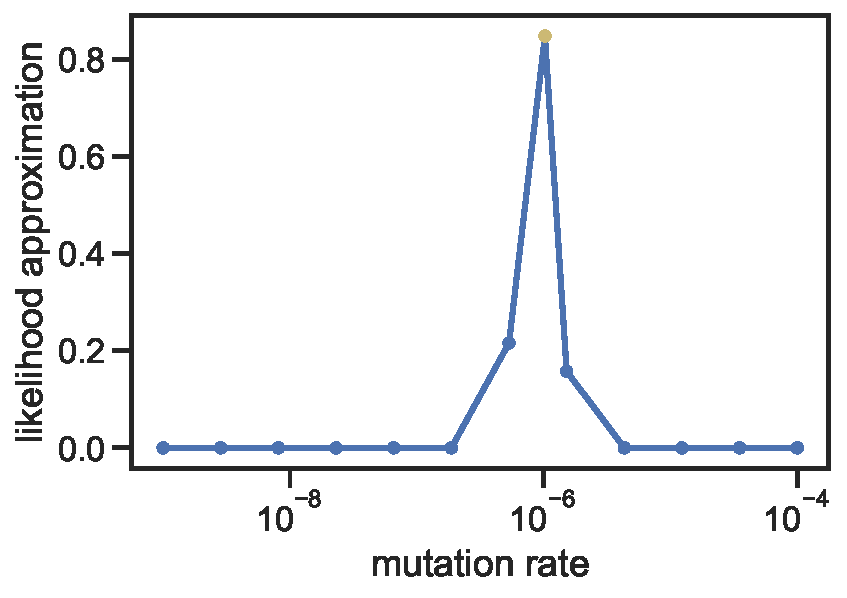
\includegraphics[width=\textwidth]{../figures/sensitivity-mutation-rate-plot.pdf}      
      \label{fig:sensitivity-mutation}
  \end{subfigure}
  \begin{subfigure}{0.3\textwidth}
      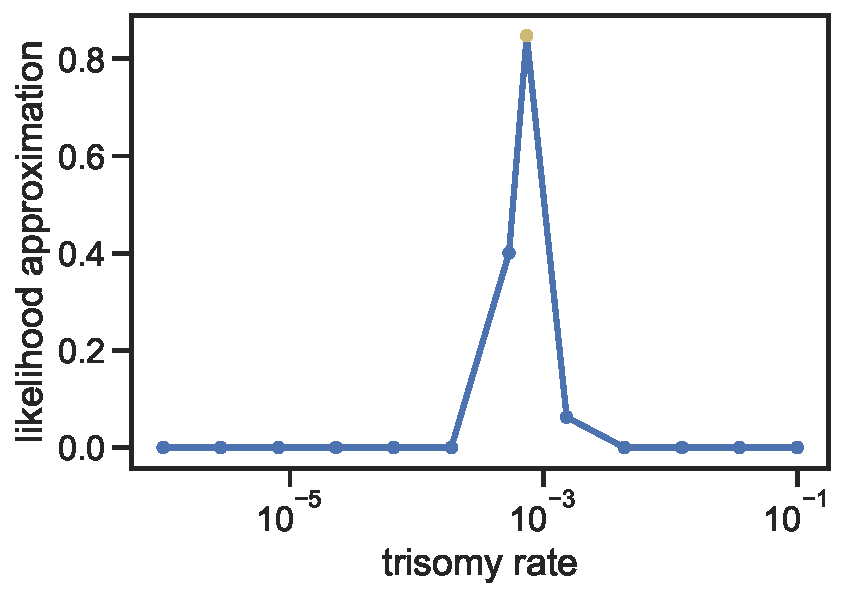
\includegraphics[width=\textwidth]{../figures/sensitivity-trisomy-rate-plot.pdf}      
      \label{fig:sensitivity-aneuploidy}
  \end{subfigure}
   \begin{subfigure}{0.3\textwidth}
      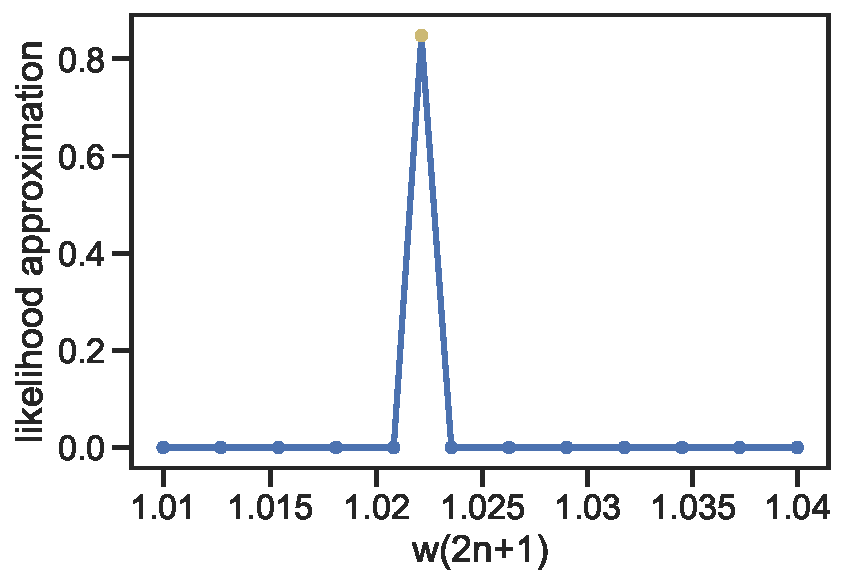
\includegraphics[width=\textwidth]{../figures/sensitivity-w(2n+1)-plot.pdf}      
      \label{fig:sensitivity-anwt}
  \end{subfigure}
    \begin{subfigure}{0.3\textwidth}
      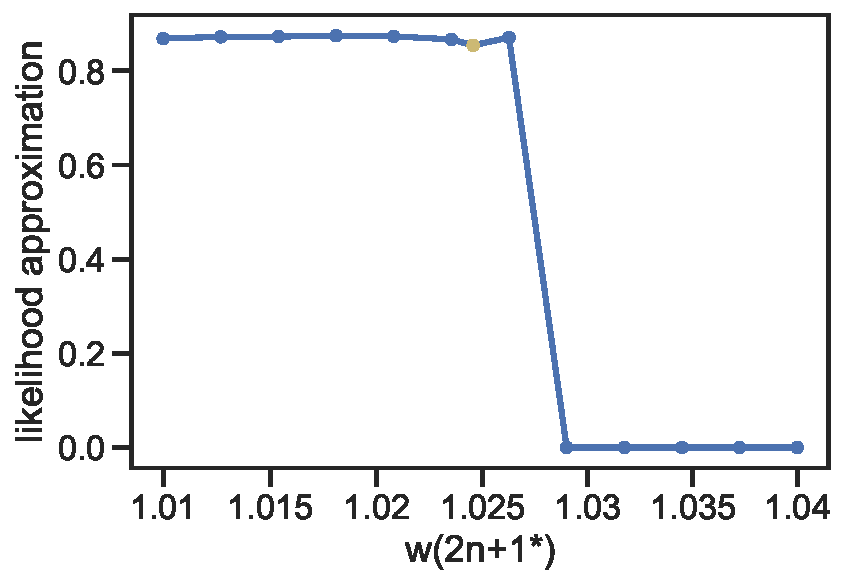
\includegraphics[width=\textwidth]{../figures/sensitivity-w(2n+1*)-plot.pdf}      
      \label{fig:sensitivity-anmt}
  \end{subfigure}
    \begin{subfigure}{0.3\textwidth}
      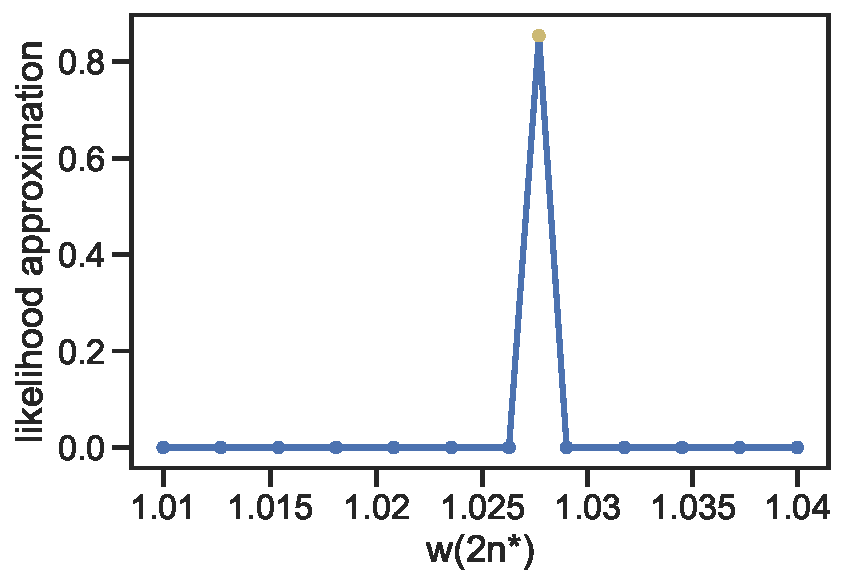
\includegraphics[width=\textwidth]{../figures/sensitivity-w(2n*)-plot.pdf}      
      \label{fig:sensitivity-eumt}
  \end{subfigure}
  \caption{
    \textbf{Sensitivity analysis.} We take parameters that are median of the posterior. Then we change only one parameter at time while measuring the model likelihood of the parameters. x-axis label represent the parameter that we change. Yellow point indicates the median value.
  }
  \label{fig:sensitivity}
\end{figure}

\end{document}  